\begin{algorithm}[hbtp]
\caption{Aggregating communities into super-vertices \cite{sahu2023gvelouvain}.}
\label{alg:louvainag}
\begin{algorithmic}[1]
\Require{$G'$: Input/super-vertex graph}
\Require{$C'$: Community membership of each vertex}
\Ensure{$G'_{C'}$: Community vertices (CSR)}
\Ensure{$G''$: Super-vertex graph (weighted CSR)}
\Ensure{$*.offsets$: Offsets array of a CSR graph}
\Ensure{$H_t$: Collision-free per-thread hashtable}

\Statex

\Function{louvainAggregate}{$G', C'$}
  \State $\rhd$ Obtain vertices belonging to each community
  \State $G'_{C'}.offsets \gets countCommunityVertices(G', C')$ \label{alg:louvainag--coff-begin}
  \State $G'_{C'}.offsets \gets exclusiveScan(G'_{C'}.offsets)$ \label{alg:louvainag--coff-end}
  \ForAll{$i \in V'$ \textbf{in parallel}} \label{alg:louvainag--comv-begin}
    \State Add edge $(C'[i], i)$ to CSR $G'_{C'}$ atomically
  \EndFor \label{alg:louvainag--comv-end}
  \State $\rhd$ Obtain super-vertex graph
  \State $G''.offsets \gets communityTotalDegree(G', C')$ \label{alg:louvainag--yoff-begin}
  \State $G''.offsets \gets exclusiveScan(G''.offsets)$ \label{alg:louvainag--yoff-end}
  \State $|\Gamma| \gets$ Number of communities in $C'$
  \ForAll{$c \in [0, |\Gamma|)$ \textbf{in parallel}} \label{alg:louvainag--y-begin}
    \If{degree of $c$ in $G'_{C'} = 0$} \textbf{continue}
    \EndIf
    \State $H_t \gets \{\}$
    \ForAll{$i \in G'_{C'}.edges(c)$}
      \State $H_t \gets scanCommunities(H, G', C', i, true)$
    \EndFor
    \ForAll{$(d, w) \in H_t$}
      \State Add edge $(c, d, w)$ to CSR $G''$ atomically
    \EndFor
  \EndFor \label{alg:louvainag--y-end}
  \Return $G''$ \label{alg:louvainag--return}
\EndFunction
\end{algorithmic}
\end{algorithm}

\begin{algorithm}[hbtp]
\caption{Updating vertex/community weights \cite{sahu2023gvelouvain}.}
\label{alg:louvainag}
\begin{algorithmic}[1]
\Require{$G'$: Input/super-vertex graph}
\Require{$C'$: Community membership of each vertex}
\Ensure{$G'_{C'}$: Community vertices (CSR)}
\Ensure{$G''$: Super-vertex graph (weighted CSR)}
\Ensure{$*.offsets$: Offsets array of a CSR graph}
\Ensure{$H_t$: Collision-free per-thread hashtable}

\Statex

\Function{louvainUpdateWeights}{$G^t, \Delta^{t-}, \Delta^{t+}, C^{t-1}, K^{t-1}, \Sigma^{t-1}$}
  \State $K \gets K^{t-1}$ \textbf{;} $\Sigma \gets \Sigma^{t-1}$
  \ForAll{\textbf{threads in parallel}}
    \ForAll{$(i, j, w) \in \Delta^{t-}$}
      \State $c \gets C[i]$
      \If{$i \in work_{th}$} $K[i] \gets K[i] - w$
      \EndIf
      \If{$c \in work_{th}$} $\Sigma[c] \gets \Sigma[c] - w$
      \EndIf
    \EndFor
    \ForAll{$(i, j, w) \in \Delta^{t+}$}
      \State $c \gets C[i]$
      \If{$i \in work_{th}$} $K[i] \gets K[i] + w$
      \EndIf
      \If{$c \in work_{th}$} $\Sigma[c] \gets \Sigma[c] + w$
      \EndIf
    \EndFor
  \EndFor
  \Return $K, \Sigma$
\EndFunction
\end{algorithmic}
\end{algorithm}




\subsection{Correctness of DF Louvain}
\label{sec:louvain-correctness}

We now provide arguments for the correctness of Dynamic Frontier (DF) Louvain. To help with this, we refer the reader to Figure \ref{fig:frontier-approach}. Here, pre-existing edges are represented by solid lines, and $i$ represents a source vertex of edge deletions/insertions in the batch update. Edge deletions in the batch update with $i$ as the source vertex are shown in the top row (denoted by dashed lines), edge insertions are shown in the middle row (also denoted by dashed lines), and community migration of vertex $i$ is is shown in the bottom row. Vertices $i_n$ and $j_n$ represent the destination vertices (of edge deletions or insertions). Vertices $i'$, $j'$, and $k'$ signify neighboring vertices of vertex $i$. Finally, vertices $i''$, $j''$, and $k''$ represent non-neighbor vertices (to vertex $i$). Yellow highlighting is used to indicate vertices marked as affected, initially or in the current iteration of the community detection algorithm. We understand this figure is dense, but we tried to capture several details for the correctness arguments.

Given a batch update consisting of edge deletions $\Delta^{t-}$ and insertions $\Delta^{t+}$, we now show that DF Louvain marks the essential vertices, which have an incentive to change their community membership, as affected. For any given vertex $i$ in the original graph (before the batch update), the delta-modularity of moving it from its current community $d$ to a new community $c$ is given by Equation \ref{eq:delta-modularity-clone}. We now consider the direct effect of each individual edge deletion $(i, j)$ or insertion $(i, j, w)$ in the batch update, on the delta-modularity of the a vertex, as well as the indirect cascading effect of migration of a vertex (to another community) on other vertices.

\begin{equation}
\label{eq:delta-modularity-clone}
  \Delta Q_{i: d \rightarrow c}
  = \frac{1}{m} (K_{i \rightarrow c} - K_{i \rightarrow d}) - \frac{K_i}{2m^2} (K_i + \Sigma_c - \Sigma_d)
\end{equation}

\begin{figure}[hbtp]
  \centering
  \subfigure{
    \label{fig:dynamic-frontier-detailed}
    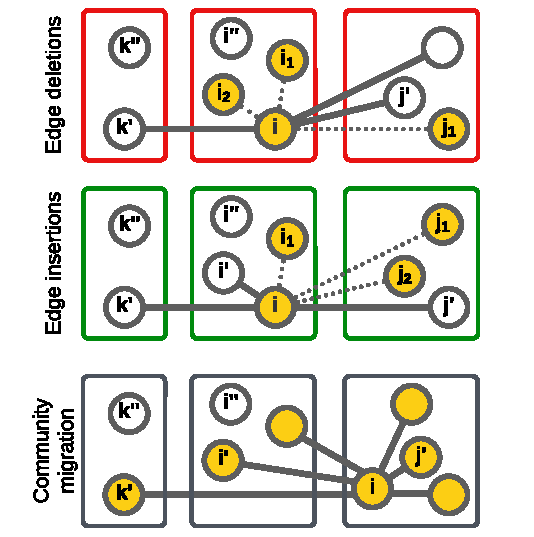
\includegraphics[width=0.78\linewidth]{out/about-frontier-detail.pdf}
  } \\[-2ex]
  \caption{A detailed illustration for presenting arguments on the correctness of \textit{Dynamic Frontier (DF)} Louvain.}
  \label{fig:frontier-approach}
\end{figure}





\subsubsection{On edge deletion}

\begin{lemma}
\label{thm:louvain--mark-deletion}
Given an edge deletion $(i, j)$ between vertices $i$ and $j$ belonging to the same community $d$, vertex $i$ (and $j$) should be marked as affected.
\end{lemma}

Consider the case of edge deletion $(i, j)$ of weight $w$ between vertices $i$ and $j$ belonging to the same community $C_i = C_j = d$ (see Figure \ref{fig:frontier-approach}, where $j = i_1$). Let $i''$ be a vertex belonging $i$'s community $C_{i''} = d$, and let $k''$ be a vertex belonging to another community $C_{k''} = b$. As shown below in Case \textbf{(1)}, the delta-modularity of vertex $i$ moving from its original community $d$ to another community $b$ has a significant positive factor $w/m$. There is thus a chance that vertex $i$ would change its community membership, and we should mark it as affected. The same argument applies for vertex $j$, as the edge is undirected. On the other hand, for the Cases \textbf{(2)}-\textbf{(3)}, there is only a small positive change in delta-modularity for vertex $k''$. Thus, there is little incentive for vertex $k''$ to change its community membership, and no incentive for a change in community membership of vertex $i''$.

Note that it is possible that the community $d$ would split due to the edge deletion. However, this is unlikely, given that one would need a large number of edge deletions between vertices belonging to the same community for the community to split. With DF Louvain, such rare events are taken care of\ignore{One can take care of such rare events} by running Static Louvain every \verb|RESTART_LOUVAIN|\ignore{$1000$} batch updates, which also helps us ensure high-quality communities. The same applies to $\Delta$-screening ($\Delta S$) Louvain.

\begin{enumerate}
  \item $\Delta Q_{i:d \rightarrow b}^{new} = \Delta Q_{i:d \rightarrow b} + [\frac{w}{m}] + \frac{w}{2m^2} (\Sigma_c - \Sigma_d + w)$
  \item $\Delta Q_{i'':d \rightarrow b}^{new} = \Delta Q_{i'':d \rightarrow b} - \frac{wK_{i''}}{m^2}$
  \item $\Delta Q_{k'':b \rightarrow d}^{new} = \Delta Q_{k'':b \rightarrow d} + \frac{wK_{k''}}{m^2}$
\end{enumerate}

Now, consider the case of edge deletion $(i, j)$ between vertices $i$ and $j$ belonging to different communities, i.e., $C_i = d$, $C_j = c$ (see Figure \ref{fig:frontier-approach}, where $j = j_2$ or $j_3$). Let $i''$ be a vertex belonging to $i$'s community $C_{i''} = d$, $j''$ be a vertex belonging to $j$'s community $C_{j''} = c$, and $k''$ be a vertex belonging another community $C_{k''} = b$. As shown in Cases \textbf{(4)}-\textbf{(8)}, due to the absence of any significant positive change in delta-modularity, there is little to no incentive for vertices $i$, $j$, $k''$, $i''$, and $j''$ to change their community membership.

\begin{enumerate}[start=4]
  \item $\Delta Q_{i:d \rightarrow c}^{new} = \Delta Q_{i:d \rightarrow c} - \frac{w}{m} + \frac{w}{2m^2} (2K_i + \Sigma_c - \Sigma_d - w)$
  \item $\Delta Q_{i:d \rightarrow b}^{new} = \Delta Q_{i:d \rightarrow b} + \frac{w}{2m^2} (K_i + \Sigma_b - \Sigma_d)$
  \item $\Delta Q_{i'':d \rightarrow c}^{new} = \Delta Q_{i'':d \rightarrow c}$
  \item $\Delta Q_{i'':d \rightarrow b}^{new} = \Delta Q_{i'':d \rightarrow b} - \frac{wK_{i''}}{2m^2}$
  \item $\Delta Q_{k'':b \rightarrow d/c}^{new} = \Delta Q_{k'':b \rightarrow d/c} + \frac{wK_{k''}}{m^2}$ \hfill $\diamond$
\end{enumerate}




\subsubsection{On edge insertion}

\begin{lemma}
\label{thm:louvain--mark-insertion}
Given an edge insertion $(i, j, w)$ between vertices $i$ and $j$ belonging to different communities $d$ and $c$, vertex $i$ (and $j$) should be marked as affected.
\end{lemma}

Let us consider the case of edge insertion $(i, j, w)$ between vertices $i$ and $j$ belonging to different communities $C_i = d$ and $C_j = c$ respectively (see Figure \ref{fig:frontier-approach}, where $j = j_3$). Let $i''$ be a vertex belonging $i$'s community $C_{i''} = d$, $j''$ be a vertex belonging to $j$'s community $C_{j''} = c$, and $k''$ be a vertex belonging to another community $C_{k''} = b$. As shown below in Case \textbf{(9)}, we have a significant positive factor $w/m$ (and a small negative factor) which increases the delta-modularity of vertex $i$ moving to $j$'s community after the insertion of the edge $(i, j)$. There is, therefore, incentive for vertex $i$ to change its community membership. Accordingly, we mark $i$ as affected. Again, the same argument applies for vertex $j$, as the edge is undirected. Further, we observe from other Cases (\textbf{(10)}-\textbf{(13)}) there is only a small change in delta-modularity. Thus, there is hardly any to no incentive for a change in community membership of vertices $i''$, $j''$, and $k''$.

\begin{enumerate}[start=9]
  \item $\Delta Q_{i:d \rightarrow c}^{new} = \Delta Q_{i:d \rightarrow c} + [\frac{w}{m}] - \frac{w}{2m^2} (2K_i + \Sigma_c - \Sigma_d + w)$
  \item $\Delta Q_{i:d \rightarrow b}^{new} = \Delta Q_{i:d \rightarrow b} - \frac{w}{2m^2} (K_i + \Sigma_b - \Sigma_d)$
  \item $\Delta Q_{i'':d \rightarrow c}^{new} = \Delta Q_{i'':d \rightarrow c}$
  \item $\Delta Q_{i'':d \rightarrow b}^{new} = \Delta Q_{i'':d \rightarrow b} + \frac{wK_{i''}}{2m^2}$
  \item $\Delta Q_{k'':b \rightarrow d/c}^{new} = \Delta Q_{k'':b \rightarrow d/c} - \frac{wK_{k''}}{2m^2}$
\end{enumerate}

Now, consider the case of edge insertion $(i, j, w)$ between vertices $i$ and $j$ belonging to the same community $C_i = C_j = d$ (see Figure \ref{fig:frontier-approach}, where $j = i_1$ or $i_2$). From Cases \textbf{(14)}-\textbf{(16)}, we note that it is little to no incentive for vertices $i''$, $k''$, $i$, and $j$ to change their community membership. Note that it is possible for the insertion of edges within the same community to cause it to split into two more strongly connected communities, but it is very unlikely.

\begin{enumerate}[start=14]
  \item $\Delta Q_{i:d \rightarrow b}^{new} = \Delta Q_{i:d \rightarrow b} - \frac{w}{m} - \frac{w}{2m^2} (\Sigma_c - \Sigma_d - w)$
  \item $\Delta Q_{i'':d \rightarrow b}^{new} = \Delta Q_{i'':d \rightarrow b} + \frac{wK_{i''}}{m^2}$
  \item $\Delta Q_{k'':b \rightarrow d}^{new} = \Delta Q_{k'':b \rightarrow d} - \frac{wK_{k''}}{m^2}$ \hfill $\diamond$
\end{enumerate}




\subsubsection{On vertex migration to another community}

\begin{lemma}
\label{thm:louvain--remark}
When a vertex $i$ changes its community membership, and vertex $j$ is its neighbor, $j$ should be marked as affected.
\end{lemma}

We considered the direct effects of deletion and insertion of edges above. Now we consider its indirect effects by studying the impact of change in community membership of one vertex on the other vertices. Consider the case where a vertex $i$ changes its community membership from its previous community $d$ to a new community $c$ (see Figure \ref{fig:frontier-approach}). Let $i'$ be a neighbor of $i$ and $i''$ be a non-neighbor of $i$ belonging to $i$'s previous community $C_{i'} = C_{i''} = d$, $j'$ be a neighbor of $i$ and $j''$ be a non-neighbor of $i$ belonging to $i$'s new community $C_{j'} = C_{j''} = c$, $k'$ be a neighbor of $i$ and $k''$ be a non-neighbor of $i$ belonging to another community $C_{k'} = C_{k''} = b$. From Cases \textbf{(17)}-\textbf{(22)}, we note that neighbors $i'$ and $k'$ have an incentive to change their community membership (as thus necessitate marking), but not $j'$. However, to keep the algorithm simple, we simply mark all the neighbors of vertex $i$ as affected.

\begin{enumerate}[start=17]
  \item $\Delta Q_{i':d \rightarrow c}^{new} = \Delta Q_{i':d \rightarrow c} + [\frac{2w_{ii'}}{m}] - \frac{K_iK_{i'}}{m^2}$
  \item $\Delta Q_{i':d \rightarrow b}^{new} = \Delta Q_{i':d \rightarrow b} + [\frac{w_{ii'}}{m}] - \frac{K_iK_{i'}}{2m^2}$
  \item $\Delta Q_{j':c \rightarrow d}^{new} = \Delta Q_{j':c \rightarrow d} - \frac{2w_{ij'}}{m} + \frac{K_iK_{j'}}{m^2}$
  \item $\Delta Q_{j':c \rightarrow b}^{new} = \Delta Q_{j':c \rightarrow b} - \frac{w_{ij'}}{m} + \frac{K_iK_{j'}}{2m^2}$
  \item $\Delta Q_{k':b \rightarrow d}^{new} = \Delta Q_{k':b \rightarrow d} - \frac{w_{ik'}}{m} + \frac{K_iK_{k'}}{2m^2}$
  \item $\Delta Q_{k':b \rightarrow c}^{new} = \Delta Q_{k':b \rightarrow c} + [\frac{w_{ik'}}{m}] - \frac{K_iK_{k'}}{2m^2}$
\end{enumerate}

Further, from Cases \textbf{(23)}-\textbf{(28)}, we note that there is hardly any incentive for a change in community membership of vertices $i''$, $j''$, and $k''$. This is due to the change in delta-modularity being insignificant. There could still be an indirect cascading impact, where a common neighbor between vertices $i$ and $j$ would change its community, which could eventually cause vertex $j$ to change its community as well \cite{com-zarayeneh21}. However, this case is automatically taken care of as we perform marking of affected vertices during the community detection process.

\begin{enumerate}[start=23]
  \item $\Delta Q_{i'':d \rightarrow c}^{new} = \Delta Q_{i'':d \rightarrow c} + \frac{K_iK_{i''}}{m^2}$
  \item $\Delta Q_{i'':d \rightarrow b}^{new} = \Delta Q_{i'':d \rightarrow b} - \frac{K_iK_{i''}}{2m^2}$
  \item $\Delta Q_{j'':c \rightarrow d}^{new} = \Delta Q_{j'':c \rightarrow d} + \frac{K_iK_{j''}}{m^2}$
  \item $\Delta Q_{j'':c \rightarrow b}^{new} = \Delta Q_{j'':c \rightarrow b} + \frac{K_iK_{j''}}{2m^2}$
  \item $\Delta Q_{k'':b \rightarrow d}^{new} = \Delta Q_{k'':b \rightarrow d} + \frac{K_iK_{k''}}{2m^2}$
  \item $\Delta Q_{k'':b \rightarrow c}^{new} = \Delta Q_{k'':b \rightarrow c} - \frac{K_iK_{k''}}{2m^2}$ \hfill $\diamond$
\end{enumerate}




\subsubsection{Overall}

Finally, based on Lemmas \ref{thm:louvain--mark-deletion}, \ref{thm:louvain--mark-insertion}, and \ref{thm:louvain--remark}, we can state the following for DF Louvain.

\begin{theorem}
\label{thm:louvain}
Given a batch update, DF Louvain marks vertices having an incentive to change their community membership as affected. \qed
\end{theorem}

We note that with DF Louvain, outlier vertices may not be marked as affected even if they have the potential to change community without any direct link to vertices in the frontier. Such outliers may be weakly connected to multiple communities, and if the current community becomes weakly (or less strongly) connected, they may leave and join some other community. It may also be noted that $\Delta S$ Louvain is also an approximate approach and can miss certain outliers. In practice, however, we see little to no impact of this approximation of the affected subset of the graph on the final quality (modularity) of the communities obtained, as shown in Section \ref{sec:evaluation}.




\begin{figure*}[!hbt]
  \centering
  \subfigure[Runtime on consecutive batch updates of size $10^{-5}|E_T|$]{
    \label{fig:temporal-sx-mathoverflow--runtime5}
    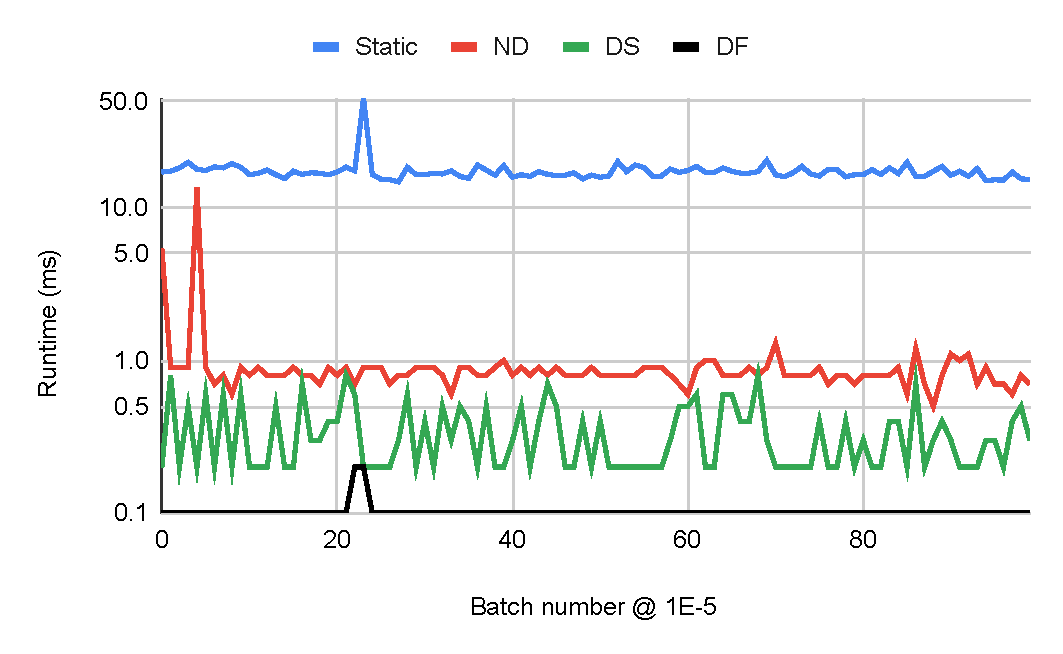
\includegraphics[width=0.48\linewidth]{out/temporal-sx-mathoverflow-runtime5.pdf}
  }
  \subfigure[Modularity in ranks obtained on consecutive batch updates of size $10^{-5}|E_T|$]{
    \label{fig:temporal-sx-mathoverflow--modularity5}
    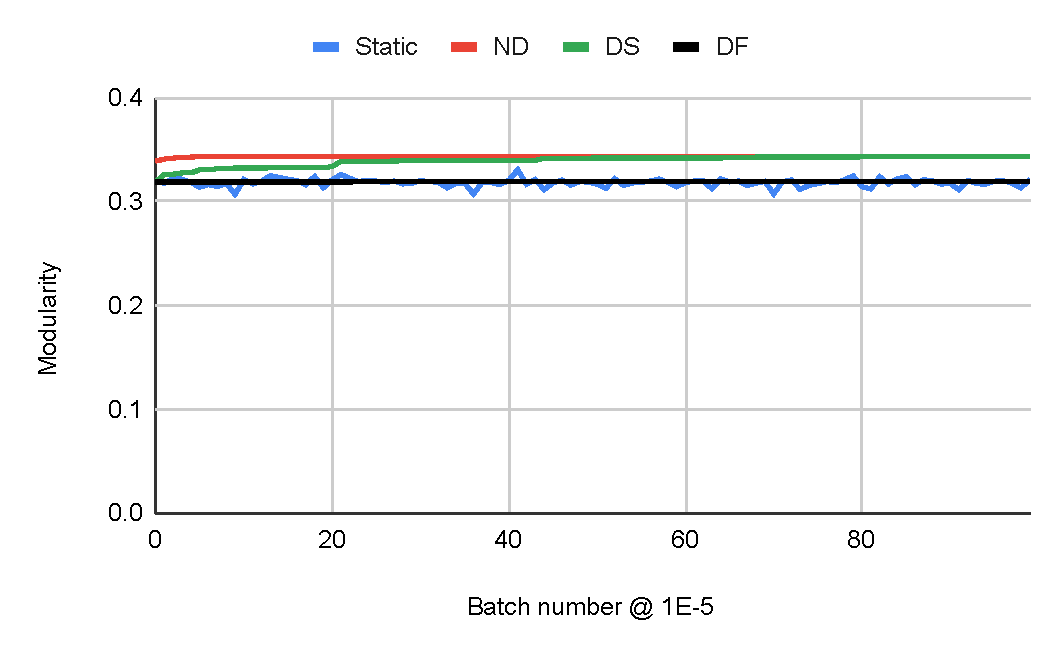
\includegraphics[width=0.48\linewidth]{out/temporal-sx-mathoverflow-modularity5.pdf}
  } \\[2ex]
  \subfigure[Runtime on consecutive batch updates of size $10^{-4}|E_T|$]{
    \label{fig:temporal-sx-mathoverflow--runtime4}
    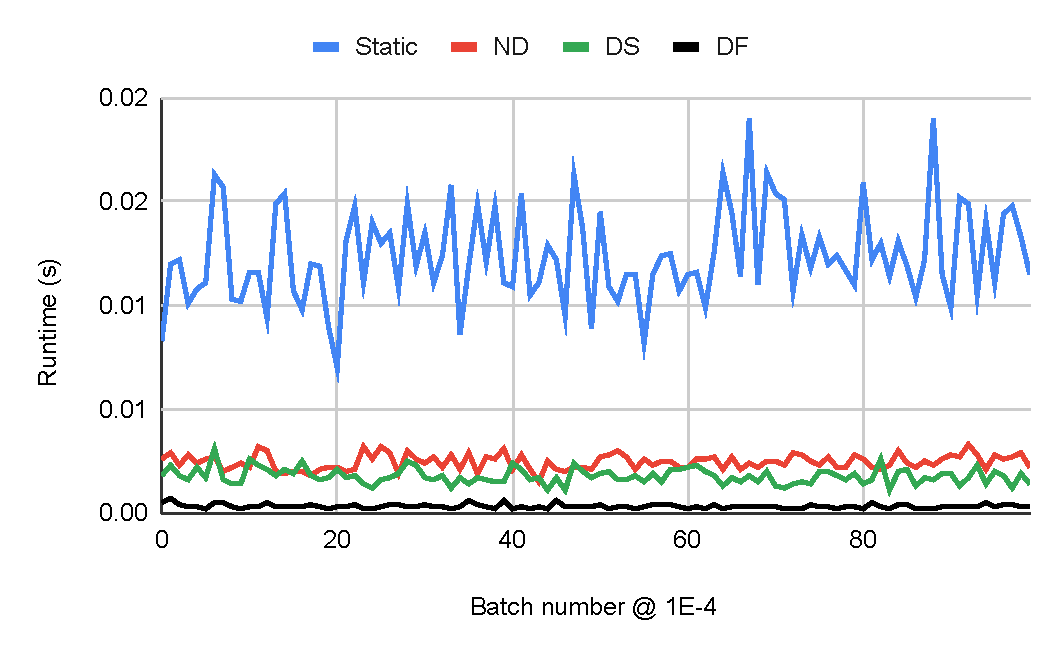
\includegraphics[width=0.48\linewidth]{out/temporal-sx-mathoverflow-runtime4.pdf}
  }
  \subfigure[Modularity in ranks obtained on consecutive batch updates of size $10^{-4}|E_T|$]{
    \label{fig:temporal-sx-mathoverflow--modularity4}
    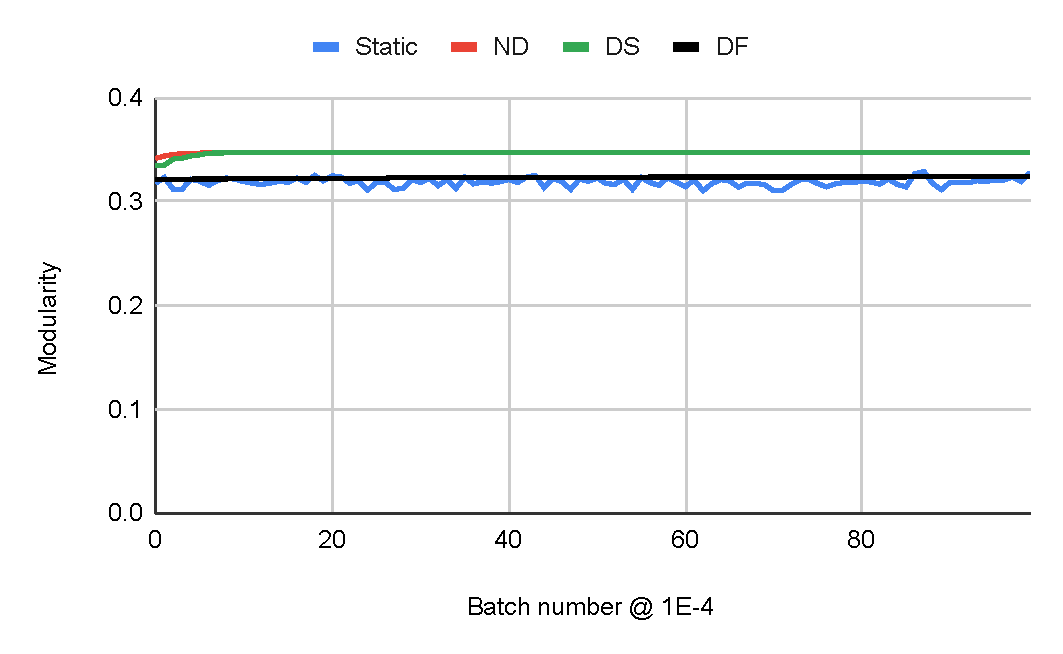
\includegraphics[width=0.48\linewidth]{out/temporal-sx-mathoverflow-modularity4.pdf}
  } \\[2ex]
  \subfigure[Runtime on consecutive batch updates of size $10^{-3}|E_T|$]{
    \label{fig:temporal-sx-mathoverflow--runtime3}
    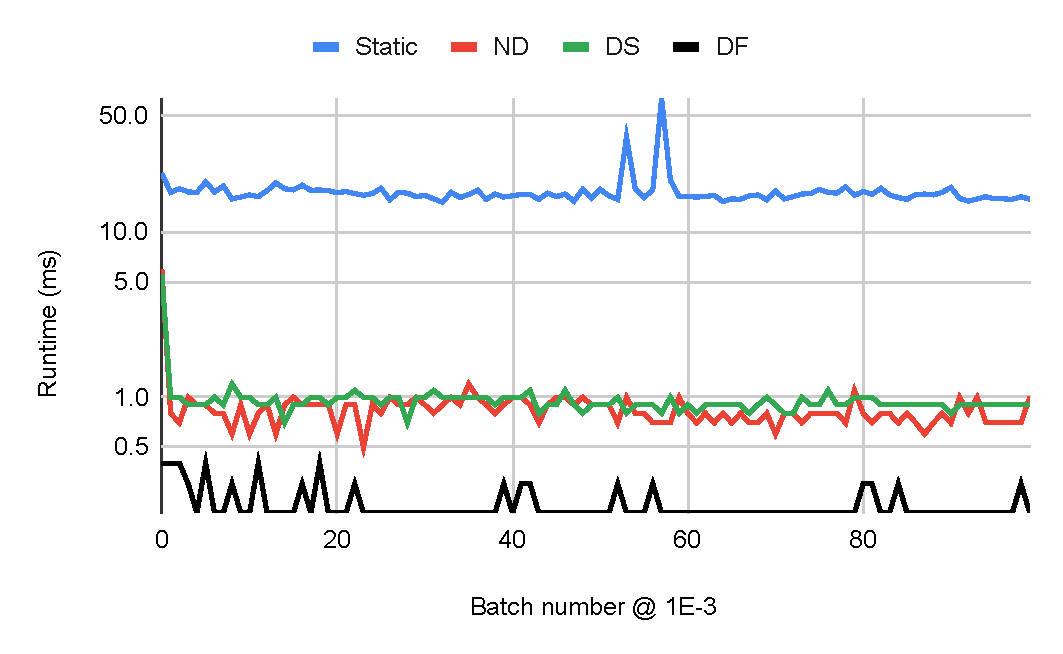
\includegraphics[width=0.48\linewidth]{out/temporal-sx-mathoverflow-runtime3.pdf}
  }
  \subfigure[Modularity in ranks obtained on consecutive batch updates of size $10^{-3}|E_T|$]{
    \label{fig:temporal-sx-mathoverflow--modularity3}
    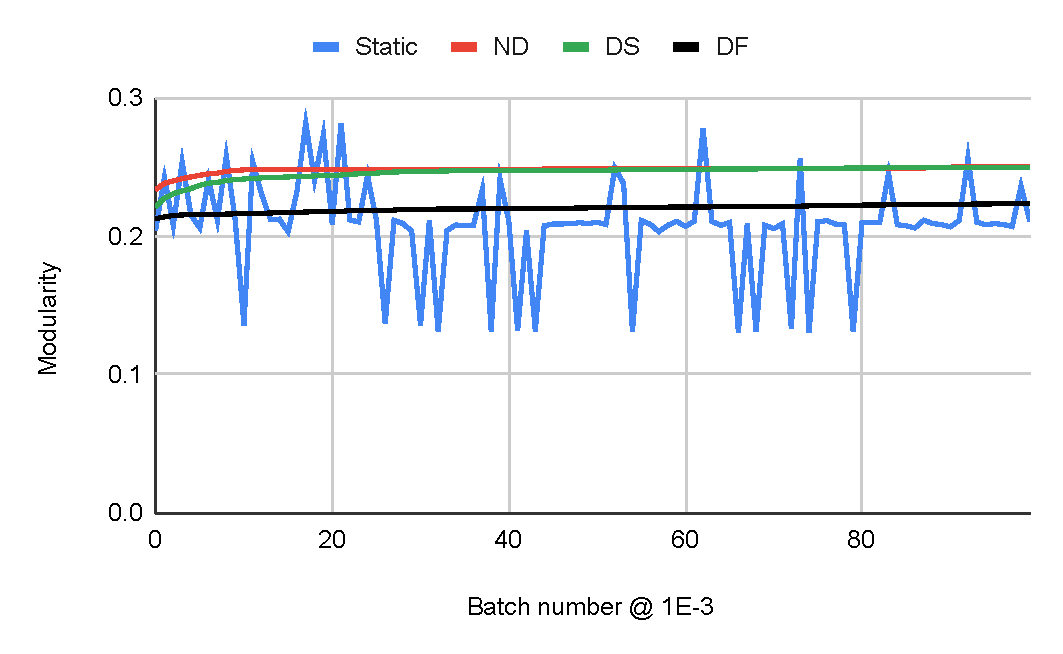
\includegraphics[width=0.48\linewidth]{out/temporal-sx-mathoverflow-modularity3.pdf}
  } \\[-2ex]
  \caption{Runtime and Modularity of communities obtained with our GPU implementation of \textit{Static}, \textit{Naive-dynamic (ND)}, \textit{Dynamic Traversal (DT)}, \textit{Dynamic Frontier (DF)}, and \textit{Dynamic Frontier with Pruning (DF-P)} PageRank on the \textit{sx-mathoverflow} dynamic graph. The size of batch updates range from $10^{-5}|E_T|$ to $10^{-3}|E_T|$. The rank modularity with each approach is measured relative to ranks obtained with a reference Static PageRank run, as detailed in Section \ref{sec:measurement}.}
  \label{fig:temporal-sx-mathoverflow}
\end{figure*}

\begin{figure*}[!hbt]
  \centering
  \subfigure[Runtime on consecutive batch updates of size $10^{-5}|E_T|$]{
    \label{fig:temporal-sx-askubuntu--runtime5}
    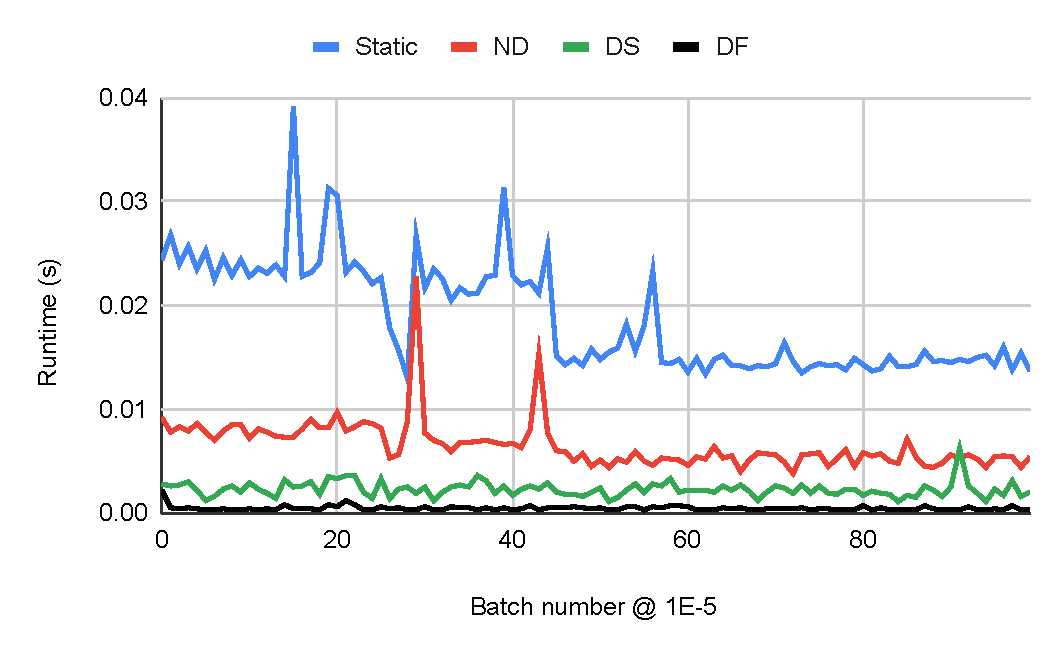
\includegraphics[width=0.48\linewidth]{out/temporal-sx-askubuntu-runtime5.pdf}
  }
  \subfigure[Modularity in ranks obtained on consecutive batch updates of size $10^{-5}|E_T|$]{
    \label{fig:temporal-sx-askubuntu--modularity5}
    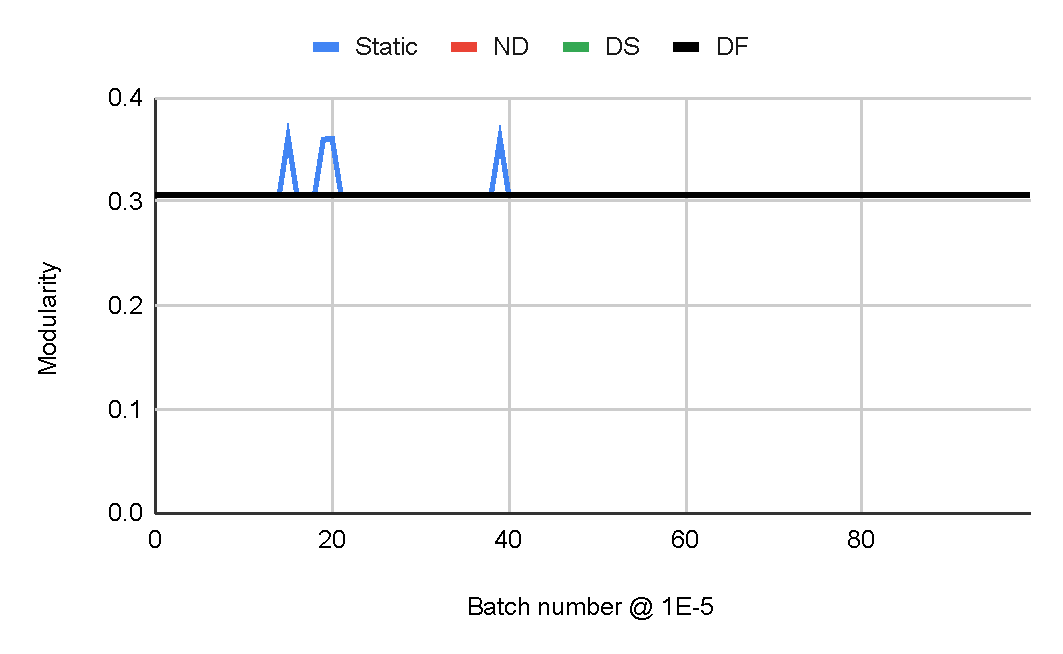
\includegraphics[width=0.48\linewidth]{out/temporal-sx-askubuntu-modularity5.pdf}
  } \\[2ex]
  \subfigure[Runtime on consecutive batch updates of size $10^{-4}|E_T|$]{
    \label{fig:temporal-sx-askubuntu--runtime4}
    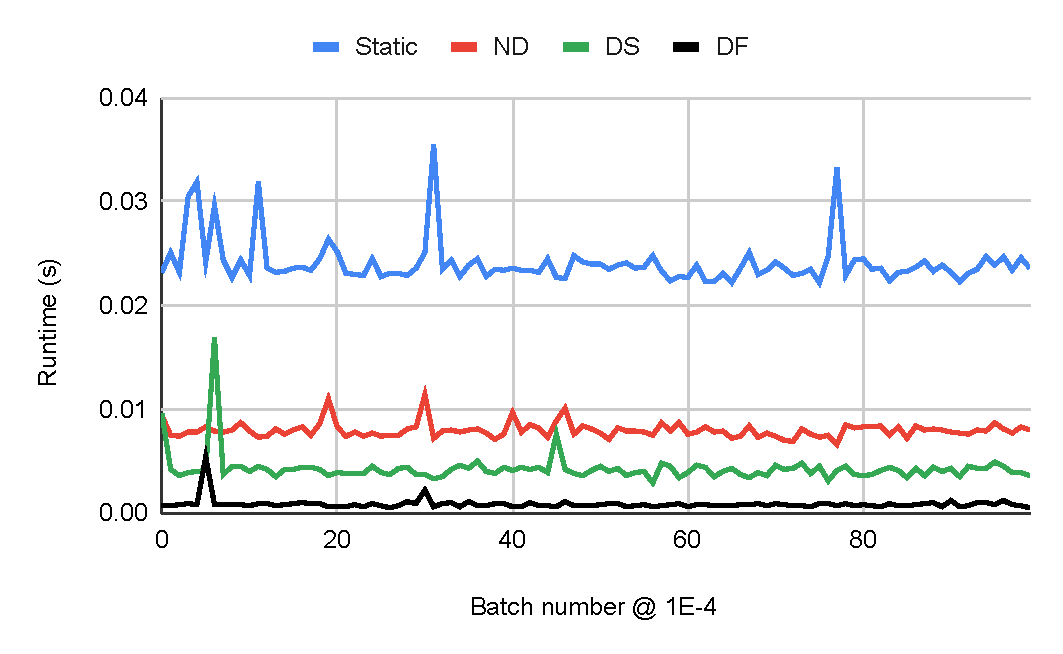
\includegraphics[width=0.48\linewidth]{out/temporal-sx-askubuntu-runtime4.pdf}
  }
  \subfigure[Modularity in ranks obtained on consecutive batch updates of size $10^{-4}|E_T|$]{
    \label{fig:temporal-sx-askubuntu--modularity4}
    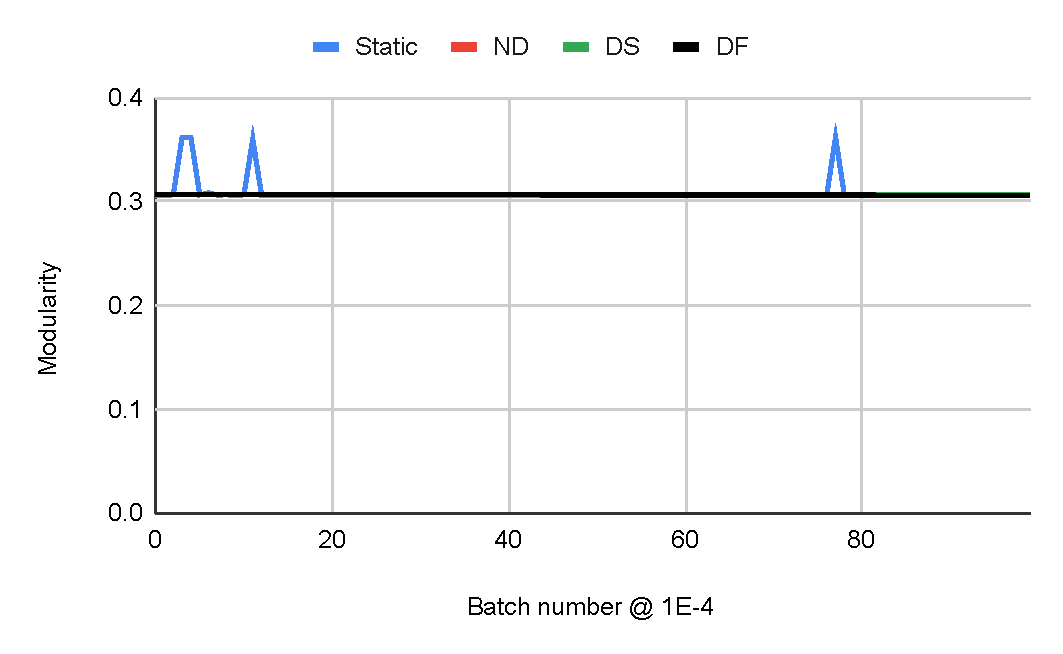
\includegraphics[width=0.48\linewidth]{out/temporal-sx-askubuntu-modularity4.pdf}
  } \\[2ex]
  \subfigure[Runtime on consecutive batch updates of size $10^{-3}|E_T|$]{
    \label{fig:temporal-sx-askubuntu--runtime3}
    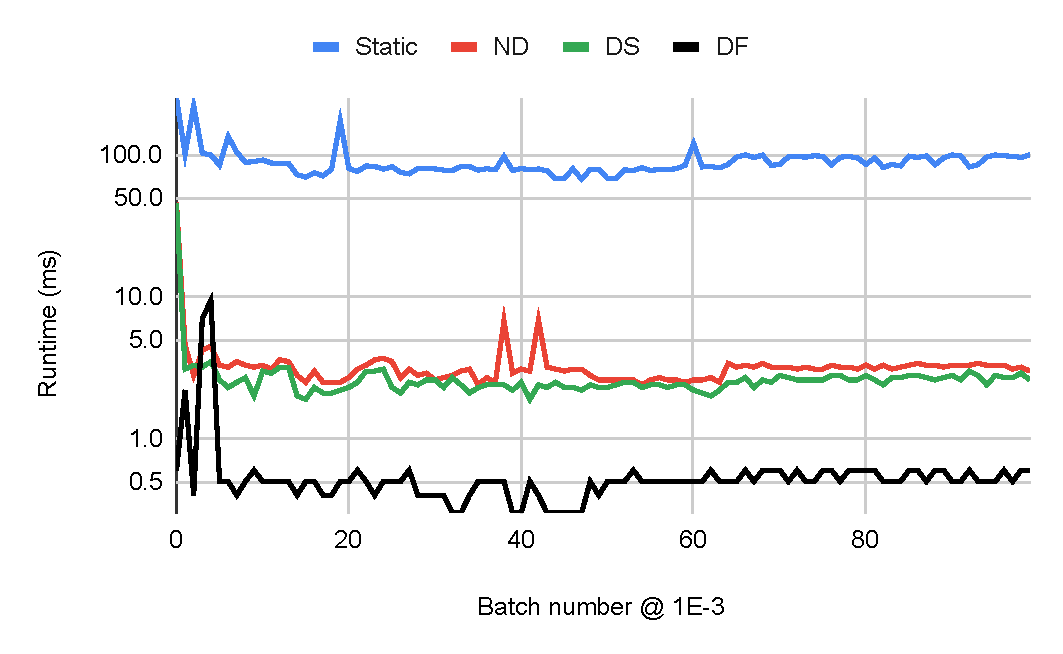
\includegraphics[width=0.48\linewidth]{out/temporal-sx-askubuntu-runtime3.pdf}
  }
  \subfigure[Modularity in ranks obtained on consecutive batch updates of size $10^{-3}|E_T|$]{
    \label{fig:temporal-sx-askubuntu--modularity3}
    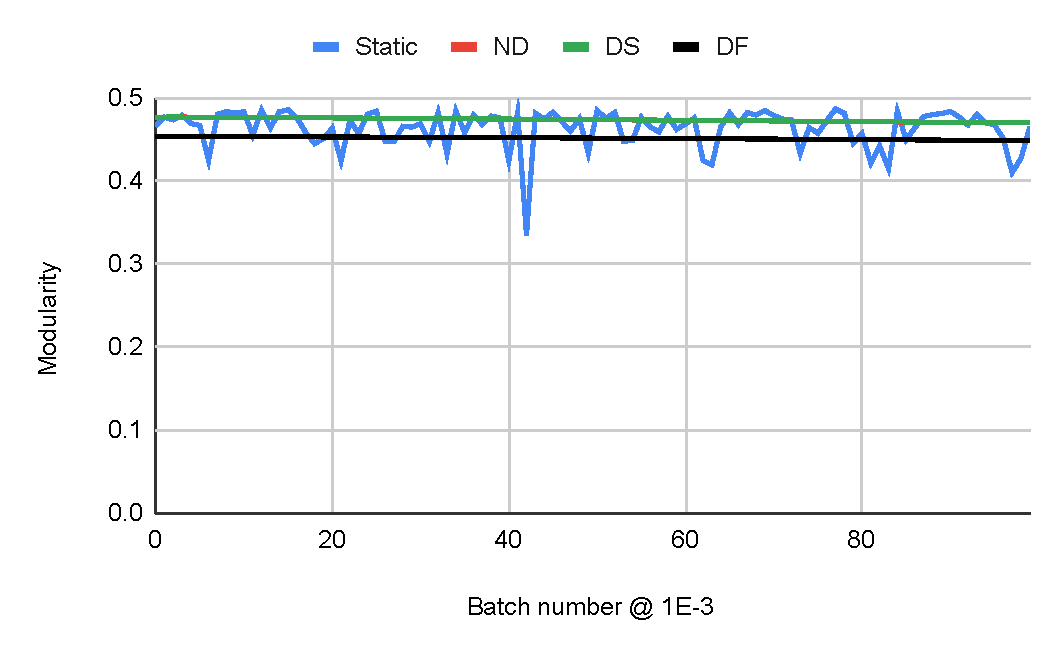
\includegraphics[width=0.48\linewidth]{out/temporal-sx-askubuntu-modularity3.pdf}
  } \\[-2ex]
  \caption{Runtime and Modularity of communities obtained with our GPU implementation of \textit{Static}, \textit{Naive-dynamic (ND)}, \textit{Dynamic Traversal (DT)}, \textit{Dynamic Frontier (DF)}, and \textit{Dynamic Frontier with Pruning (DF-P)} PageRank on the \textit{sx-askubuntu} dynamic graph. The size of batch updates range from $10^{-5}|E_T|$ to $10^{-3}|E_T|$. The rank modularity with each approach is measured relative to ranks obtained with a reference Static PageRank run, as detailed in Section \ref{sec:measurement}.}
  \label{fig:temporal-sx-askubuntu}
\end{figure*}

\begin{figure*}[!hbt]
  \centering
  \subfigure[Runtime on consecutive batch updates of size $10^{-5}|E_T|$]{
    \label{fig:temporal-sx-superuser--runtime5}
    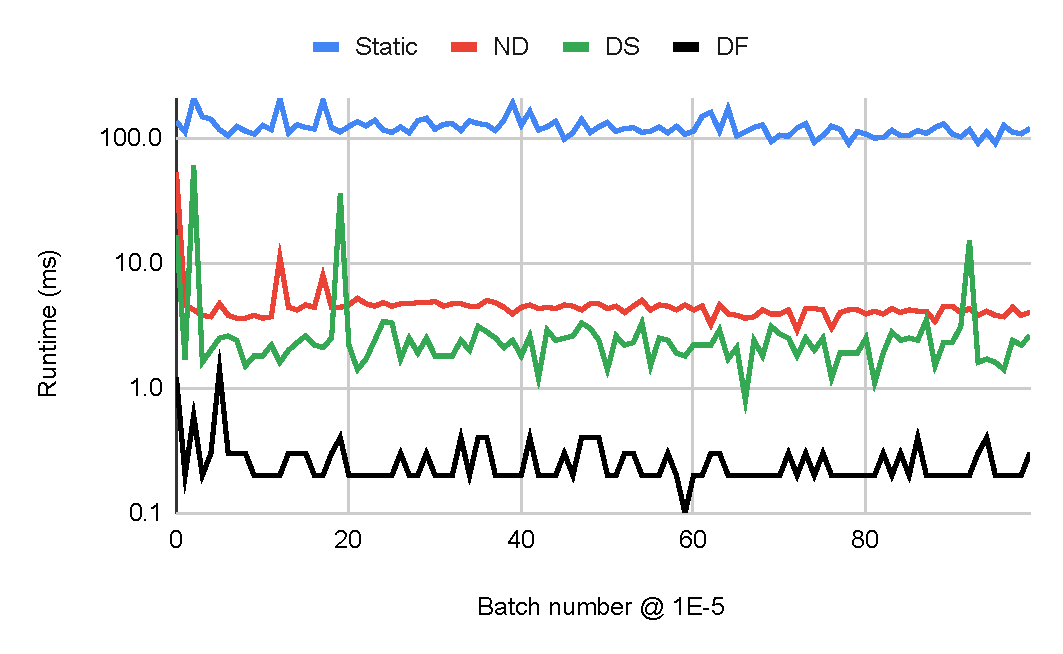
\includegraphics[width=0.48\linewidth]{out/temporal-sx-superuser-runtime5.pdf}
  }
  \subfigure[Modularity in ranks obtained on consecutive batch updates of size $10^{-5}|E_T|$]{
    \label{fig:temporal-sx-superuser--modularity5}
    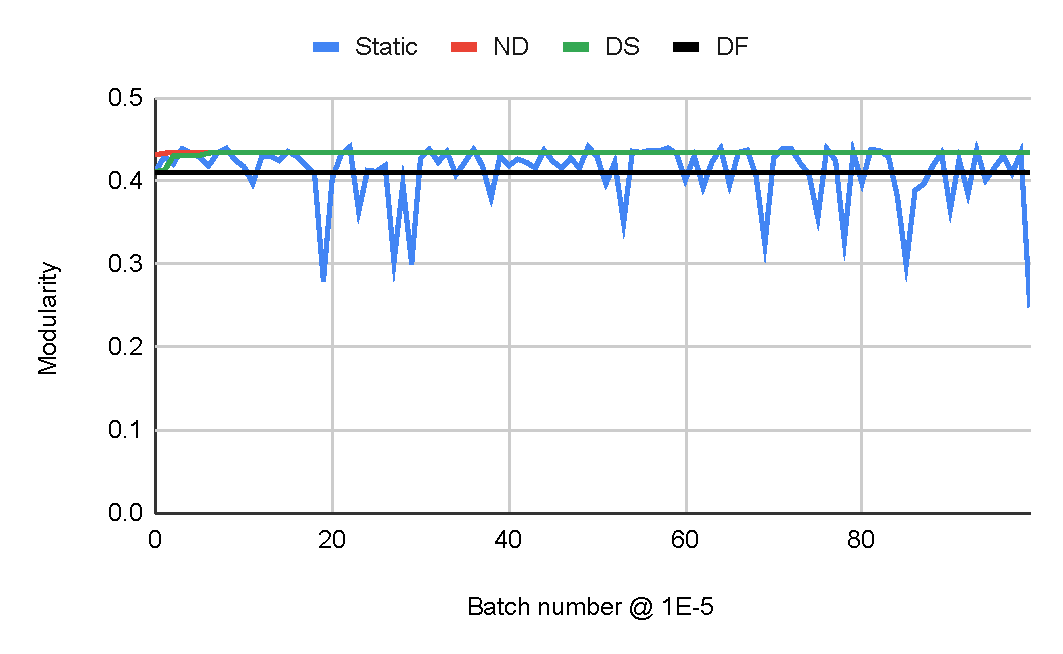
\includegraphics[width=0.48\linewidth]{out/temporal-sx-superuser-modularity5.pdf}
  } \\[2ex]
  \subfigure[Runtime on consecutive batch updates of size $10^{-4}|E_T|$]{
    \label{fig:temporal-sx-superuser--runtime4}
    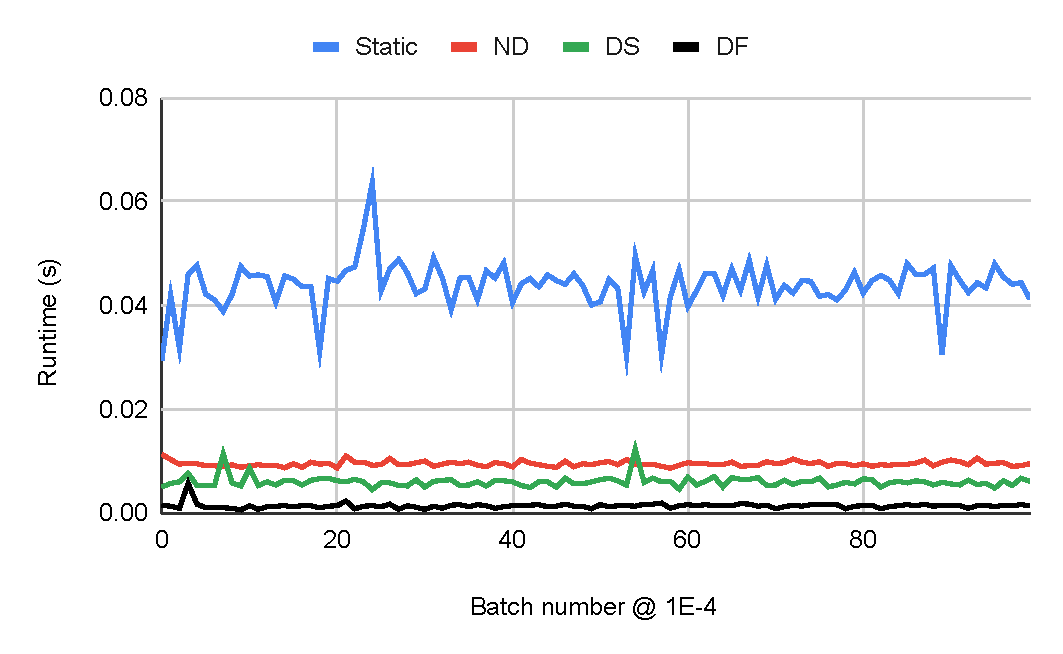
\includegraphics[width=0.48\linewidth]{out/temporal-sx-superuser-runtime4.pdf}
  }
  \subfigure[Modularity in ranks obtained on consecutive batch updates of size $10^{-4}|E_T|$]{
    \label{fig:temporal-sx-superuser--modularity4}
    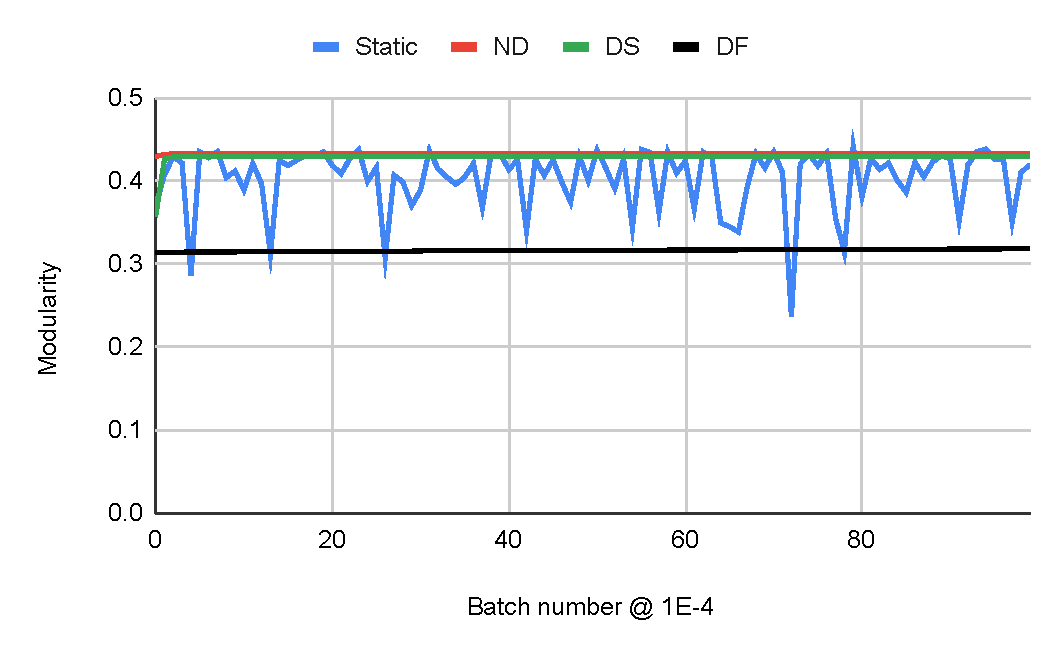
\includegraphics[width=0.48\linewidth]{out/temporal-sx-superuser-modularity4.pdf}
  } \\[2ex]
  \subfigure[Runtime on consecutive batch updates of size $10^{-3}|E_T|$]{
    \label{fig:temporal-sx-superuser--runtime3}
    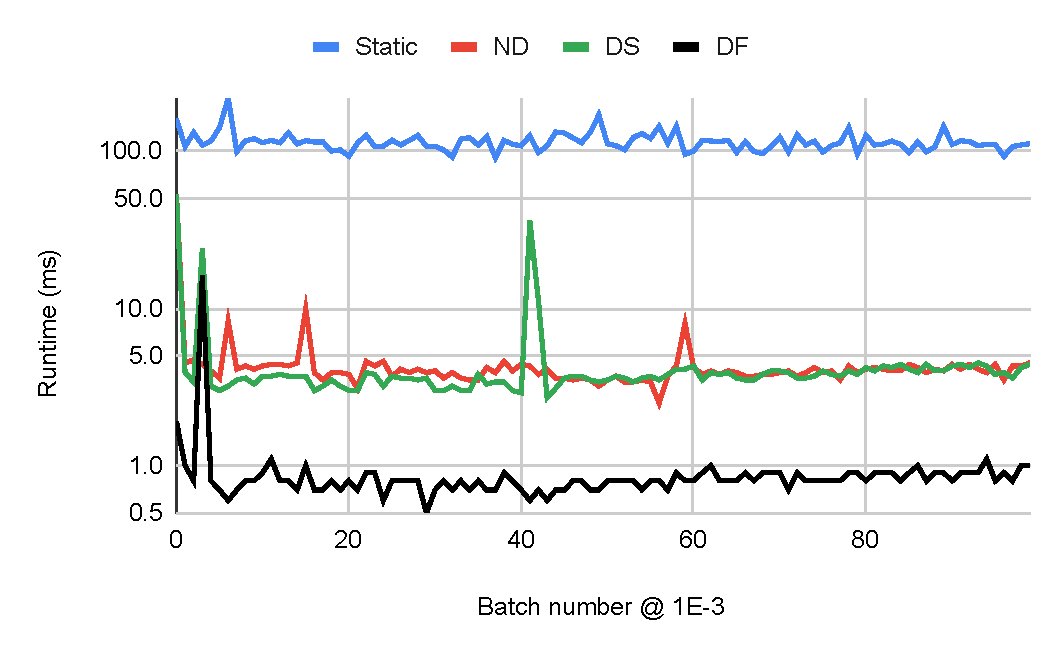
\includegraphics[width=0.48\linewidth]{out/temporal-sx-superuser-runtime3.pdf}
  }
  \subfigure[Modularity in ranks obtained on consecutive batch updates of size $10^{-3}|E_T|$]{
    \label{fig:temporal-sx-superuser--modularity3}
    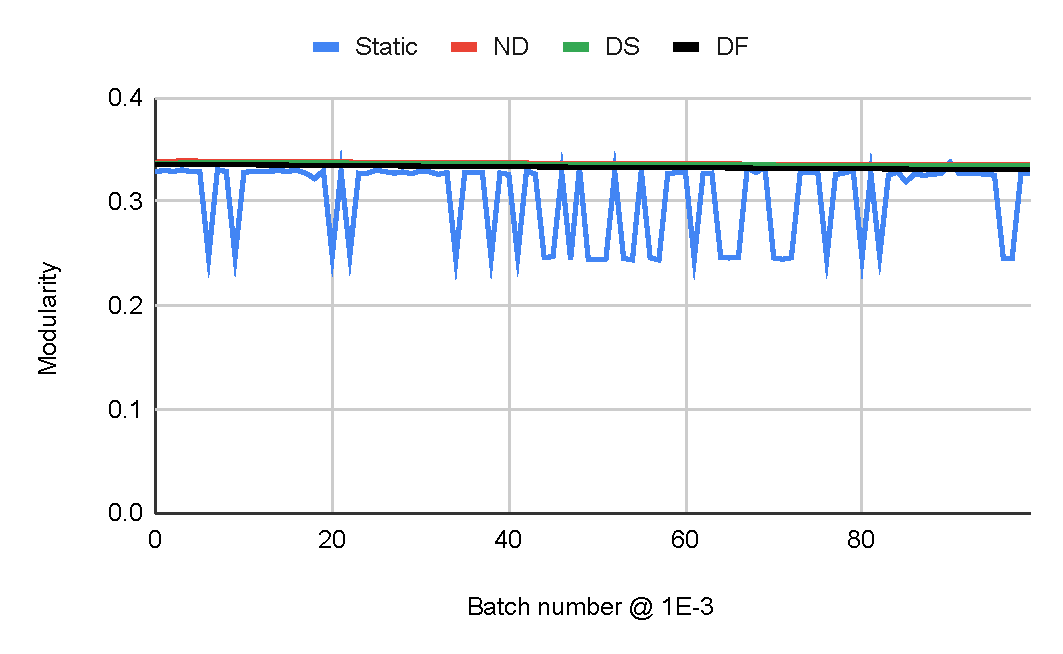
\includegraphics[width=0.48\linewidth]{out/temporal-sx-superuser-modularity3.pdf}
  } \\[-2ex]
  \caption{Runtime and Modularity of communities obtained with our GPU implementation of \textit{Static}, \textit{Naive-dynamic (ND)}, \textit{Dynamic Traversal (DT)}, \textit{Dynamic Frontier (DF)}, and \textit{Dynamic Frontier with Pruning (DF-P)} PageRank on the \textit{sx-superuser} dynamic graph. The size of batch updates range from $10^{-5}|E_T|$ to $10^{-3}|E_T|$. The rank modularity with each approach is measured relative to ranks obtained with a reference Static PageRank run, as detailed in Section \ref{sec:measurement}.}
  \label{fig:temporal-sx-superuser}
\end{figure*}

\begin{figure*}[!hbt]
  \centering
  \subfigure[Runtime on consecutive batch updates of size $10^{-5}|E_T|$]{
    \label{fig:temporal-wiki-talk-temporal--runtime5}
    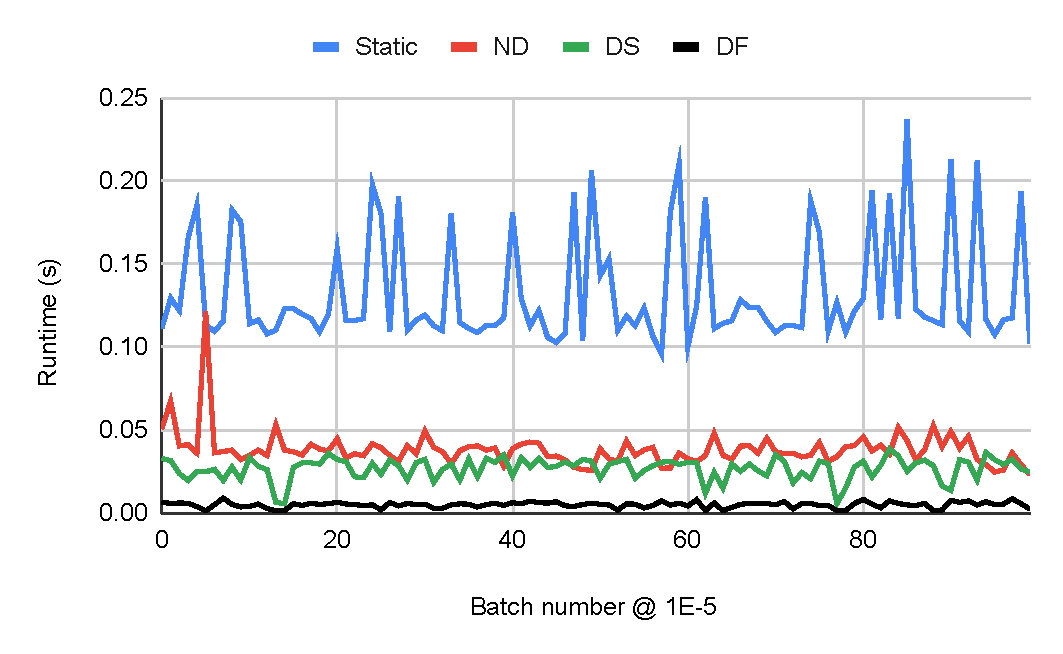
\includegraphics[width=0.48\linewidth]{out/temporal-wiki-talk-temporal-runtime5.pdf}
  }
  \subfigure[Modularity of communities obtained on consecutive batch updates of size $10^{-5}|E_T|$]{
    \label{fig:temporal-wiki-talk-temporal--modularity5}
    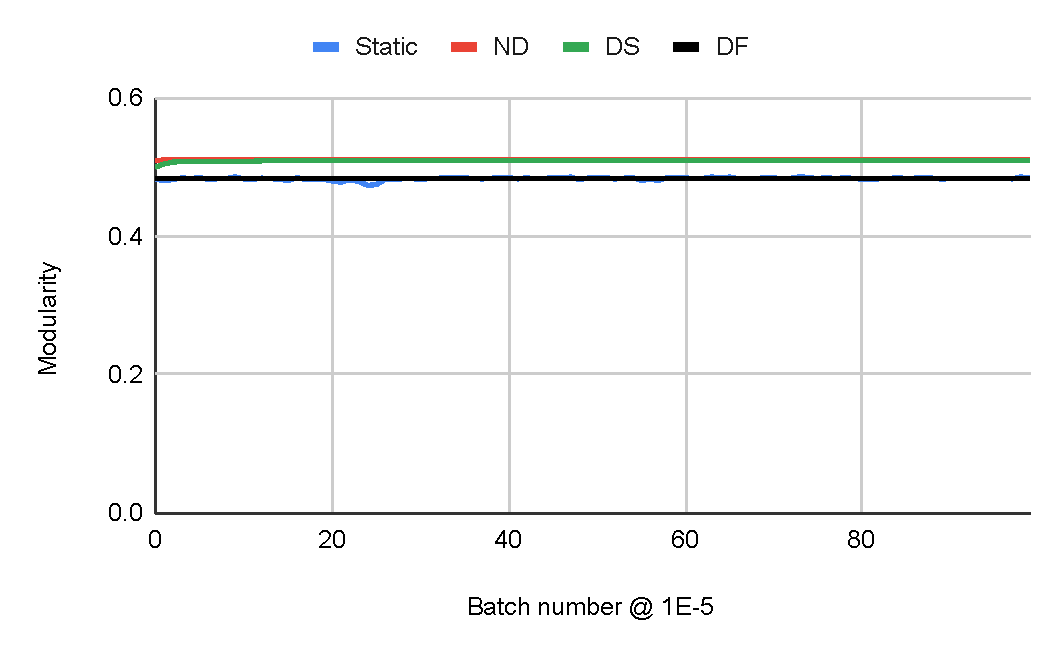
\includegraphics[width=0.48\linewidth]{out/temporal-wiki-talk-temporal-modularity5.pdf}
  } \\[2ex]
  \subfigure[Runtime on consecutive batch updates of size $10^{-4}|E_T|$]{
    \label{fig:temporal-wiki-talk-temporal--runtime4}
    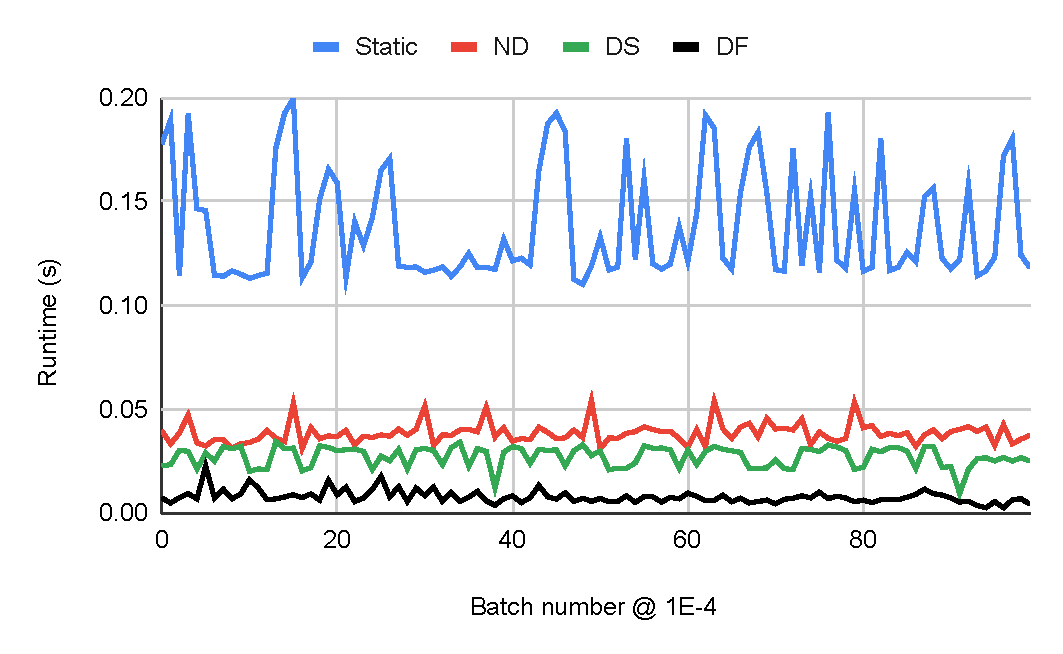
\includegraphics[width=0.48\linewidth]{out/temporal-wiki-talk-temporal-runtime4.pdf}
  }
  \subfigure[Modularity of communities obtained on consecutive batch updates of size $10^{-4}|E_T|$]{
    \label{fig:temporal-wiki-talk-temporal--modularity4}
    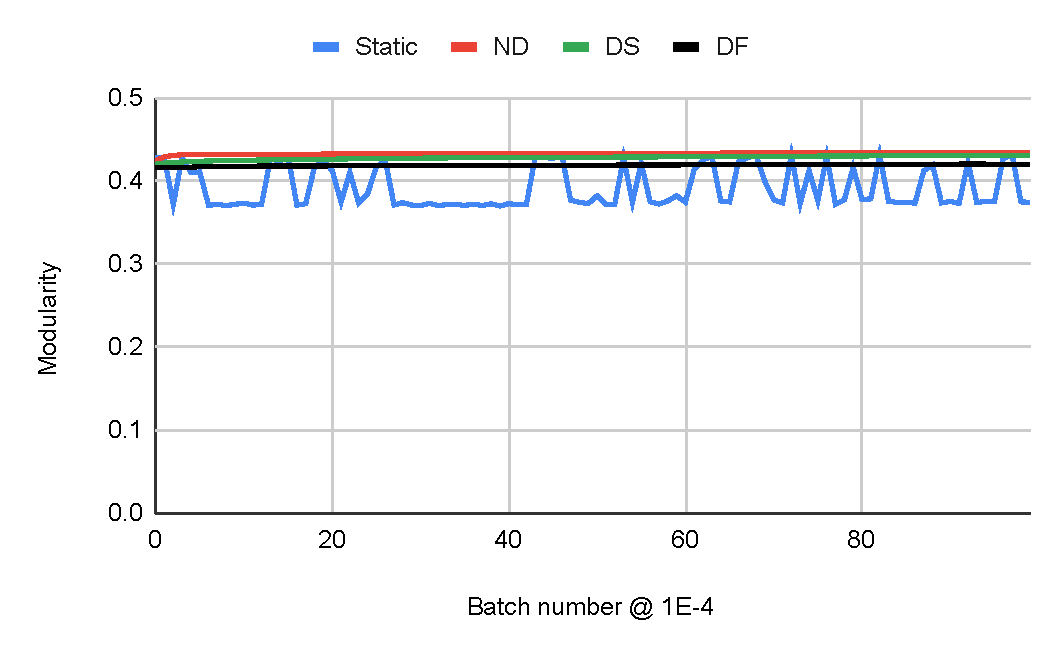
\includegraphics[width=0.48\linewidth]{out/temporal-wiki-talk-temporal-modularity4.pdf}
  } \\[2ex]
  \subfigure[Runtime on consecutive batch updates of size $10^{-3}|E_T|$]{
    \label{fig:temporal-wiki-talk-temporal--runtime3}
    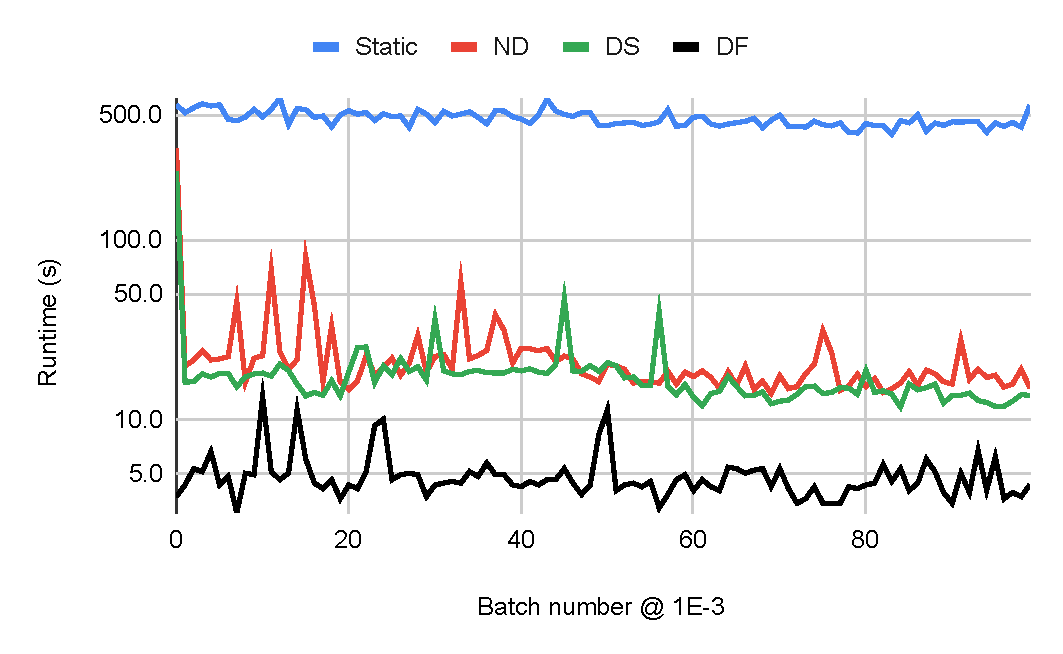
\includegraphics[width=0.48\linewidth]{out/temporal-wiki-talk-temporal-runtime3.pdf}
  }
  \subfigure[Modularity of communities obtained on consecutive batch updates of size $10^{-3}|E_T|$]{
    \label{fig:temporal-wiki-talk-temporal--modularity3}
    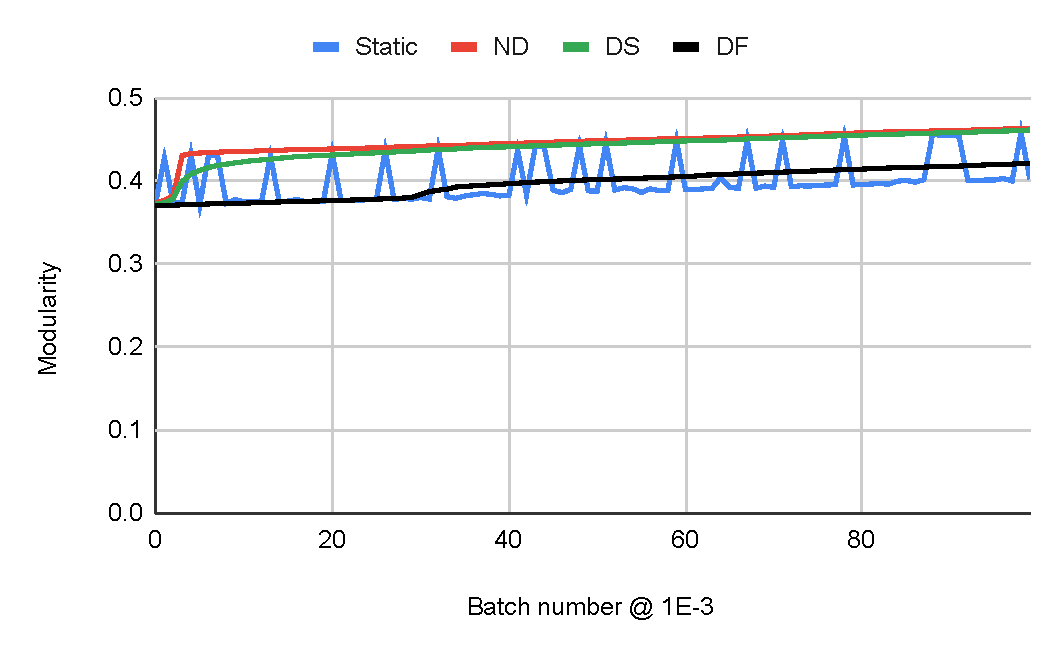
\includegraphics[width=0.48\linewidth]{out/temporal-wiki-talk-temporal-modularity3.pdf}
  } \\[-2ex]
  \caption{Runtime and Modularity of communities obtained with \textit{Static}, \textit{Naive-dynamic (ND)}, \textit{Delta-screening (DS)}, and \textit{Dynamic Frontier (DF)} Louvain on the \textit{wiki-talk-temporal} dynamic graph. The size of batch updates range from $10^{-5}|E_T|$ to $10^{-3}|E_T|$.}
  \label{fig:temporal-wiki-talk-temporal}
\end{figure*}

\begin{figure*}[!hbt]
  \centering
  \subfigure[Runtime on consecutive batch updates of size $10^{-5}|E_T|$]{
    \label{fig:temporal-sx-stackoverflow--runtime5}
    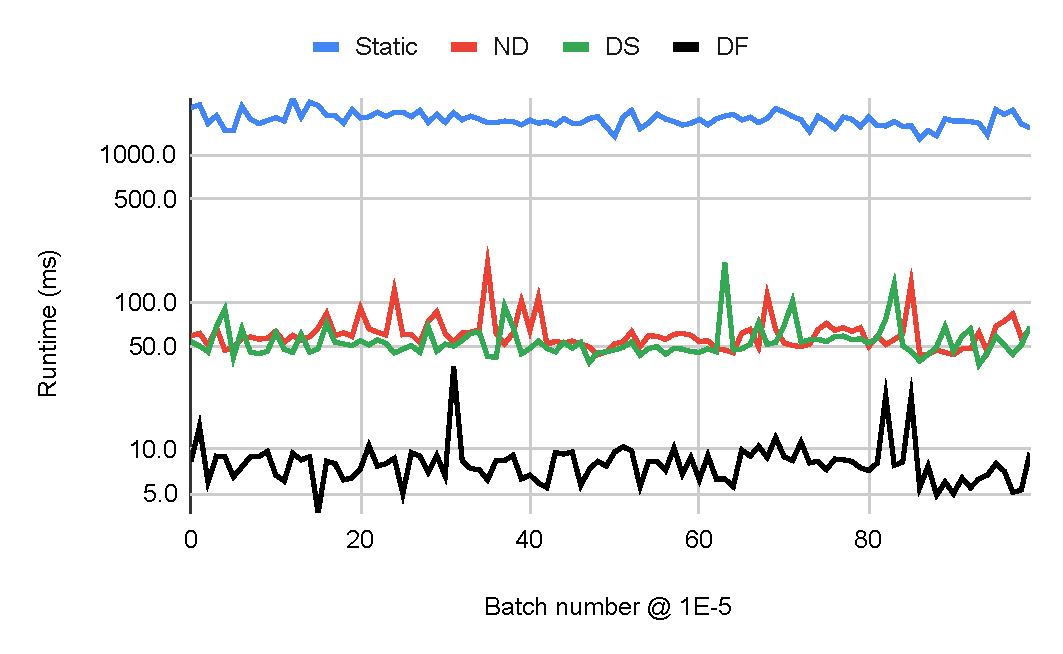
\includegraphics[width=0.48\linewidth]{out/temporal-sx-stackoverflow-runtime5.pdf}
  }
  \subfigure[Modularity in ranks obtained on consecutive batch updates of size $10^{-5}|E_T|$]{
    \label{fig:temporal-sx-stackoverflow--modularity5}
    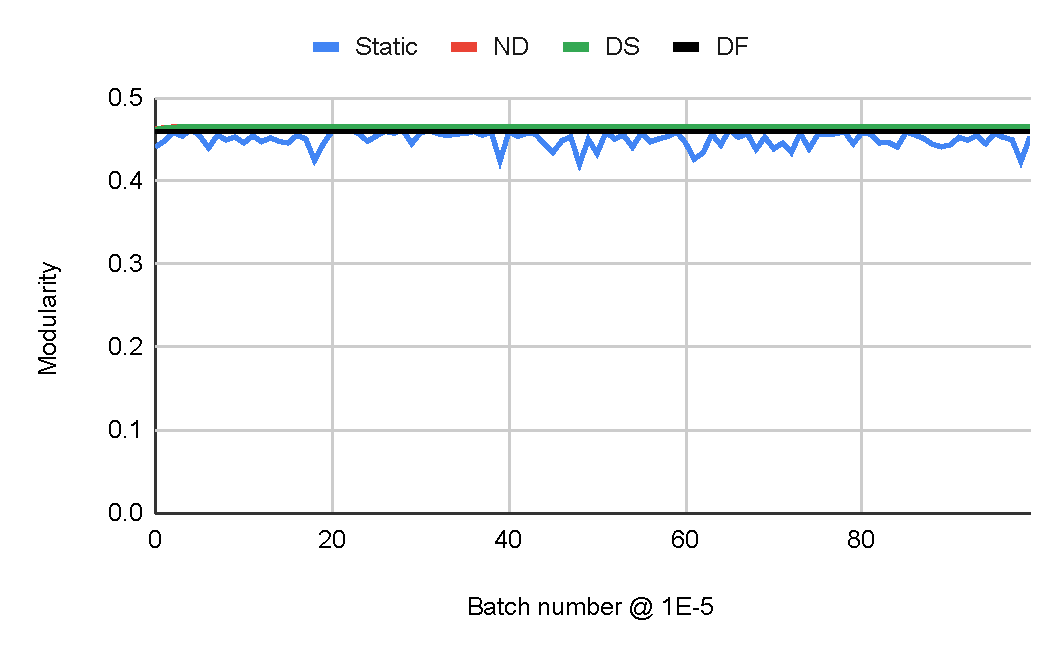
\includegraphics[width=0.48\linewidth]{out/temporal-sx-stackoverflow-modularity5.pdf}
  } \\[2ex]
  \subfigure[Runtime on consecutive batch updates of size $10^{-4}|E_T|$]{
    \label{fig:temporal-sx-stackoverflow--runtime4}
    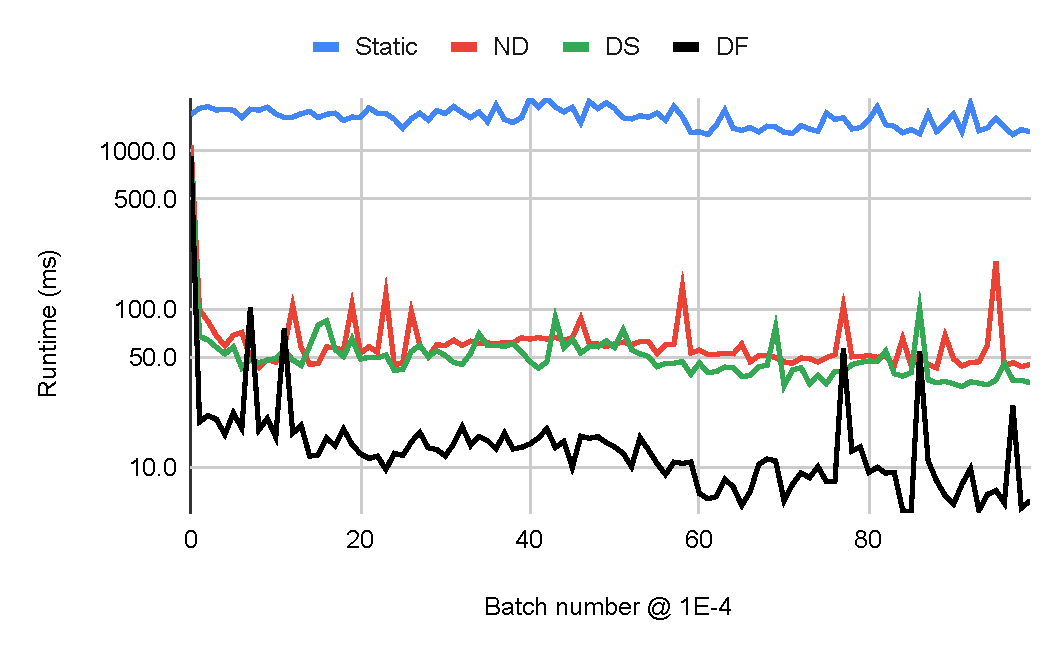
\includegraphics[width=0.48\linewidth]{out/temporal-sx-stackoverflow-runtime4.pdf}
  }
  \subfigure[Modularity in ranks obtained on consecutive batch updates of size $10^{-4}|E_T|$]{
    \label{fig:temporal-sx-stackoverflow--modularity4}
    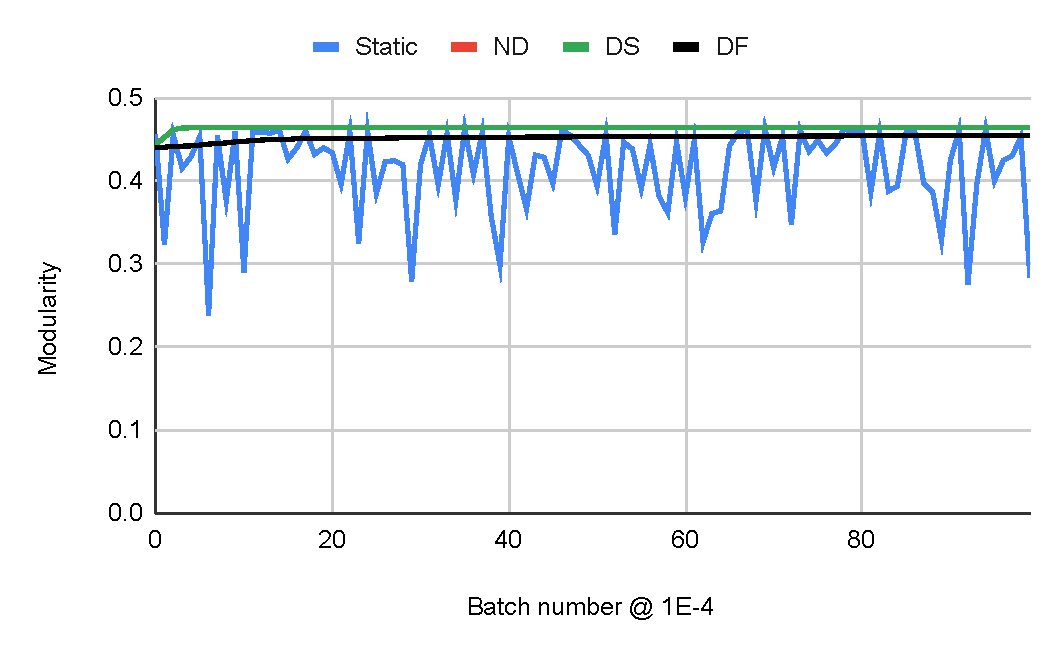
\includegraphics[width=0.48\linewidth]{out/temporal-sx-stackoverflow-modularity4.pdf}
  } \\[2ex]
  \subfigure[Runtime on consecutive batch updates of size $10^{-3}|E_T|$]{
    \label{fig:temporal-sx-stackoverflow--runtime3}
    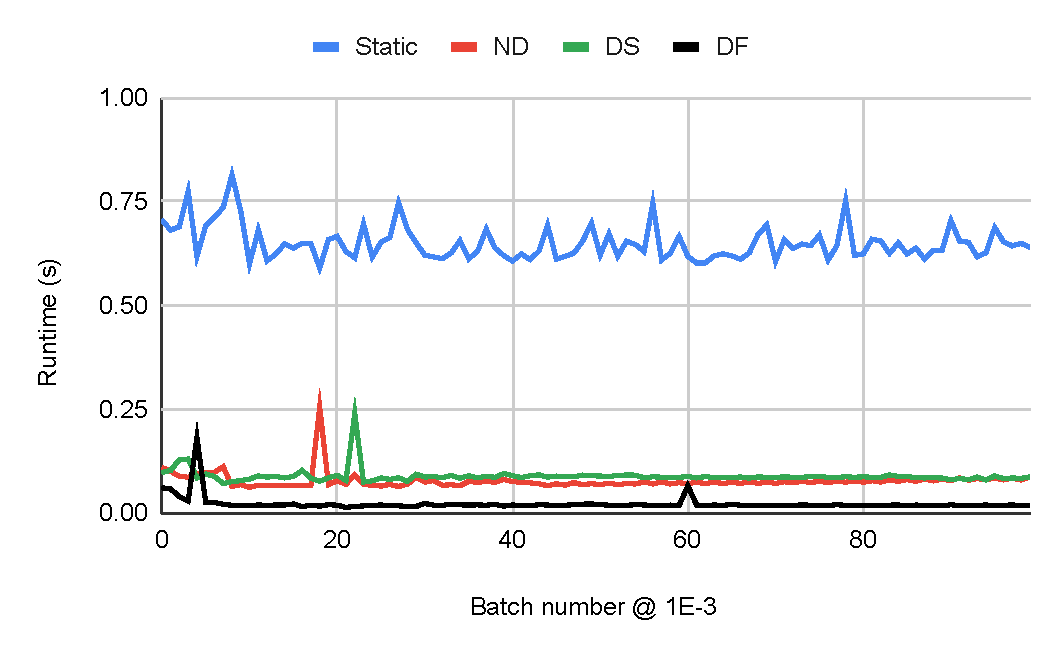
\includegraphics[width=0.48\linewidth]{out/temporal-sx-stackoverflow-runtime3.pdf}
  }
  \subfigure[Modularity in ranks obtained on consecutive batch updates of size $10^{-3}|E_T|$]{
    \label{fig:temporal-sx-stackoverflow--modularity3}
    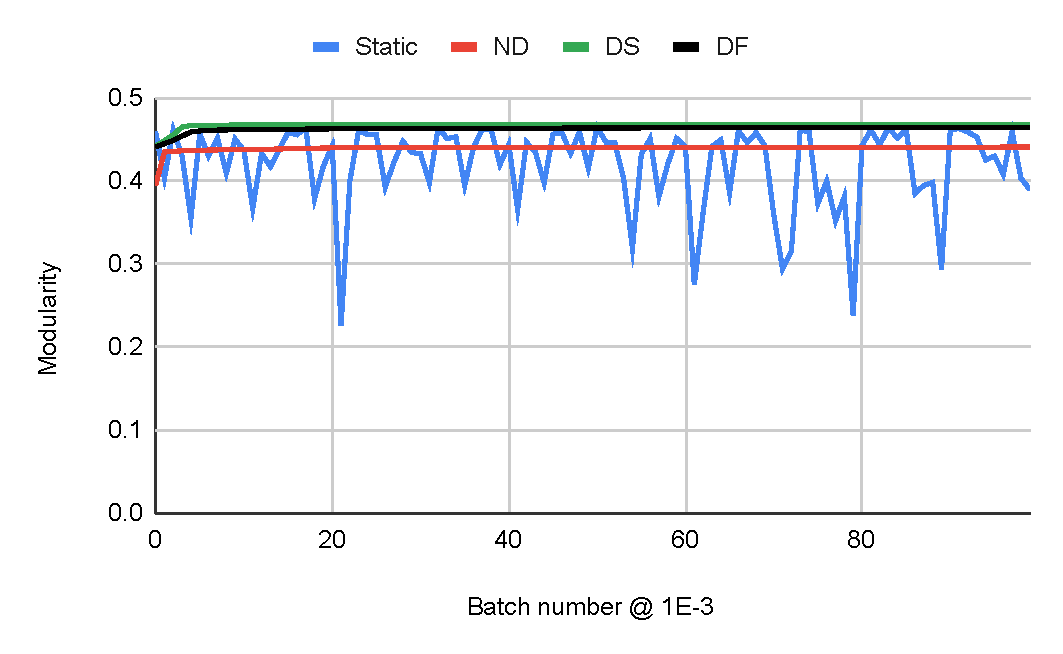
\includegraphics[width=0.48\linewidth]{out/temporal-sx-stackoverflow-modularity3.pdf}
  } \\[-2ex]
  \caption{Runtime and Modularity of communities obtained with our GPU implementation of \textit{Static}, \textit{Naive-dynamic (ND)}, \textit{Dynamic Traversal (DT)}, \textit{Dynamic Frontier (DF)}, and \textit{Dynamic Frontier with Pruning (DF-P)} PageRank on the \textit{sx-stackoverflow} dynamic graph. The size of batch updates range from $10^{-5}|E_T|$ to $10^{-3}|E_T|$. The rank modularity with each approach is measured relative to ranks obtained with a reference Static PageRank run, as detailed in Section \ref{sec:measurement}.}
  \label{fig:temporal-sx-stackoverflow}
\end{figure*}

